\documentclass[12pt,english,a4paper]{article}
\pdfobjcompresslevel=0
\usepackage[usenames,dvipsnames]{xcolor}
\usepackage[includeheadfoot,margin=0.8 in,top=0.6 in]{geometry}
\usepackage{siunitx,physics,cancel,upgreek,varioref,listings,booktabs,tocloft, pdfpages}
\usepackage{todonotes}
\usepackage{mathtools}
\usepackage{babel}
\usepackage{graphicx}
\usepackage{float}
\usepackage{fouriernc}
\usepackage{fancyhdr}
\usepackage[utf8]{inputenc}
\usepackage{amsmath}
\usepackage{amssymb}
\usepackage{textcomp}
\usepackage{lastpage}
\usepackage{microtype}
\usepackage{ifthen}
\usepackage{longtable}
\usepackage[linktoc=all, bookmarks=true, pdfauthor={Anders Johansson}]{hyperref}
\renewcommand{\CancelColor}{\color{red}}
\renewcommand{\exp}[1]{\mathrm{e}^{#1}}
\newcommand{\R}{\mathbb{R}}
\newcommand{\tittel}[1]{\title{#1 \vspace{-7ex}}\author{}\date{}\maketitle\thispagestyle{fancy}\pagestyle{fancy}\setcounter{page}{1}}

\newcommand{\deloppg}[2][]{\subsection*{#2) #1}\addcontentsline{toc}{subsection}{#2)}\refstepcounter{subsection}\label{#2}}
\newcommand{\oppg}[1]{\section*{Oppgave #1}\addcontentsline{toc}{section}{Oppgave #1}\refstepcounter{section}\label{oppg#1}}

\labelformat{section}{section~#1}
\labelformat{subsection}{section~#1}
\labelformat{subsubsection}{section~#1}
\labelformat{equation}{equation~(#1)}
\labelformat{figure}{figure~#1}
\labelformat{table}{table~#1}

\lstset{rangeprefix=/*\#,
rangesuffix=\#*/,
includerangemarker=false}
\renewcommand{\lstlistingname}{Code snippet}
\definecolor{codegreen}{rgb}{0,0.6,0}
\definecolor{codegray}{rgb}{0.5,0.5,0.5}
\definecolor{codepurple}{rgb}{0.58,0,0.82}
\definecolor{backcolour}{rgb}{0.95,0.95,0.92}
\lstset{showstringspaces=false,
basicstyle=\footnotesize\ttfamily,
keywordstyle=\color{codegreen},
commentstyle=\color{magenta},
numberstyle=\tiny\color{codegray},
stringstyle=\color{codepurple},
frameshape={RYRYNYYYY}{yny}{yny}{RYRYNYYYY},
breaklines=true,
%literate={0}{{\textcolor{blue}{0}}}{1}%
%             {1}{{\textcolor{blue}{1}}}{1}%
%             {2}{{\textcolor{blue}{2}}}{1}%
%             {3}{{\textcolor{blue}{3}}}{1}%
%             {4}{{\textcolor{blue}{4}}}{1}%
%             {5}{{\textcolor{blue}{5}}}{1}%
%             {6}{{\textcolor{blue}{6}}}{1}%
%             {7}{{\textcolor{blue}{7}}}{1}%
%             {8}{{\textcolor{blue}{8}}}{1}%
%             {9}{{\textcolor{blue}{9}}}{1}%
%             {.0}{{\textcolor{blue}{.0}}}{2}% Following is to ensure that only periods
%             {.1}{{\textcolor{blue}{.1}}}{2}% followed by a digit are changed.
%             {.2}{{\textcolor{blue}{.2}}}{2}%
%             {.3}{{\textcolor{blue}{.3}}}{2}%
%             {.4}{{\textcolor{blue}{.4}}}{2}%
%             {.5}{{\textcolor{blue}{.5}}}{2}%
%             {.6}{{\textcolor{blue}{.6}}}{2}%
%             {.7}{{\textcolor{blue}{.7}}}{2}%
%             {.8}{{\textcolor{blue}{.8}}}{2}%
%             {.9}{{\textcolor{blue}{.9}}}{2}%
}

\renewcommand{\footrulewidth}{\headrulewidth}
\tocloftpagestyle{fancy}

\setcounter{secnumdepth}{4}
\renewcommand{\thesection}{\arabic{section}}
\renewcommand{\thesubsection}{\arabic{section}.\arabic{subsection}}
\renewcommand{\thesubsubsection}{\arabic{section}.\arabic{subsection}.\arabic{subsubsection}}
\setlength{\parindent}{0cm}
\setlength{\parskip}{1em}

\newcommand{\eqtag}[1]{\refstepcounter{equation}\tag{\theequation}\label{#1}}
\hypersetup{colorlinks=true,urlcolor=blue,linkcolor=black}

\sisetup{detect-all}
\sisetup{exponent-product = \cdot, output-product = \cdot,per-mode=symbol}
\sisetup{output-decimal-marker={.}}
\sisetup{round-mode = off, round-precision=3}
\sisetup{number-unit-product = \ }
\DeclareSIUnit\year{yr}

\allowdisplaybreaks[4]
\fancyhf{}

\rhead{Kristine B. Hein and Anders Johansson}
\rfoot{Page \thepage{} of \pageref{LastPage}}
\lhead{FYS3150}
%
\usepackage[backend=biber,citestyle=numeric-comp,bibstyle=numeric,sorting=none]{biblatex}
\DefineBibliographyStrings{norsk}{%
  bibliography = {Referanser},
}
\DefineBibliographyStrings{english}{%
  bibliography = {References},
}
\addbibresource{latex/kilder.bib}

\newcommand{\program}[1]{\href{https://github.com/anjohan/Project5/blob/master/#1}{#1}}


\title{FYS3150 Project 4}
\author{Kristine Baluka Hein and Anders Johansson}
\begin{document}
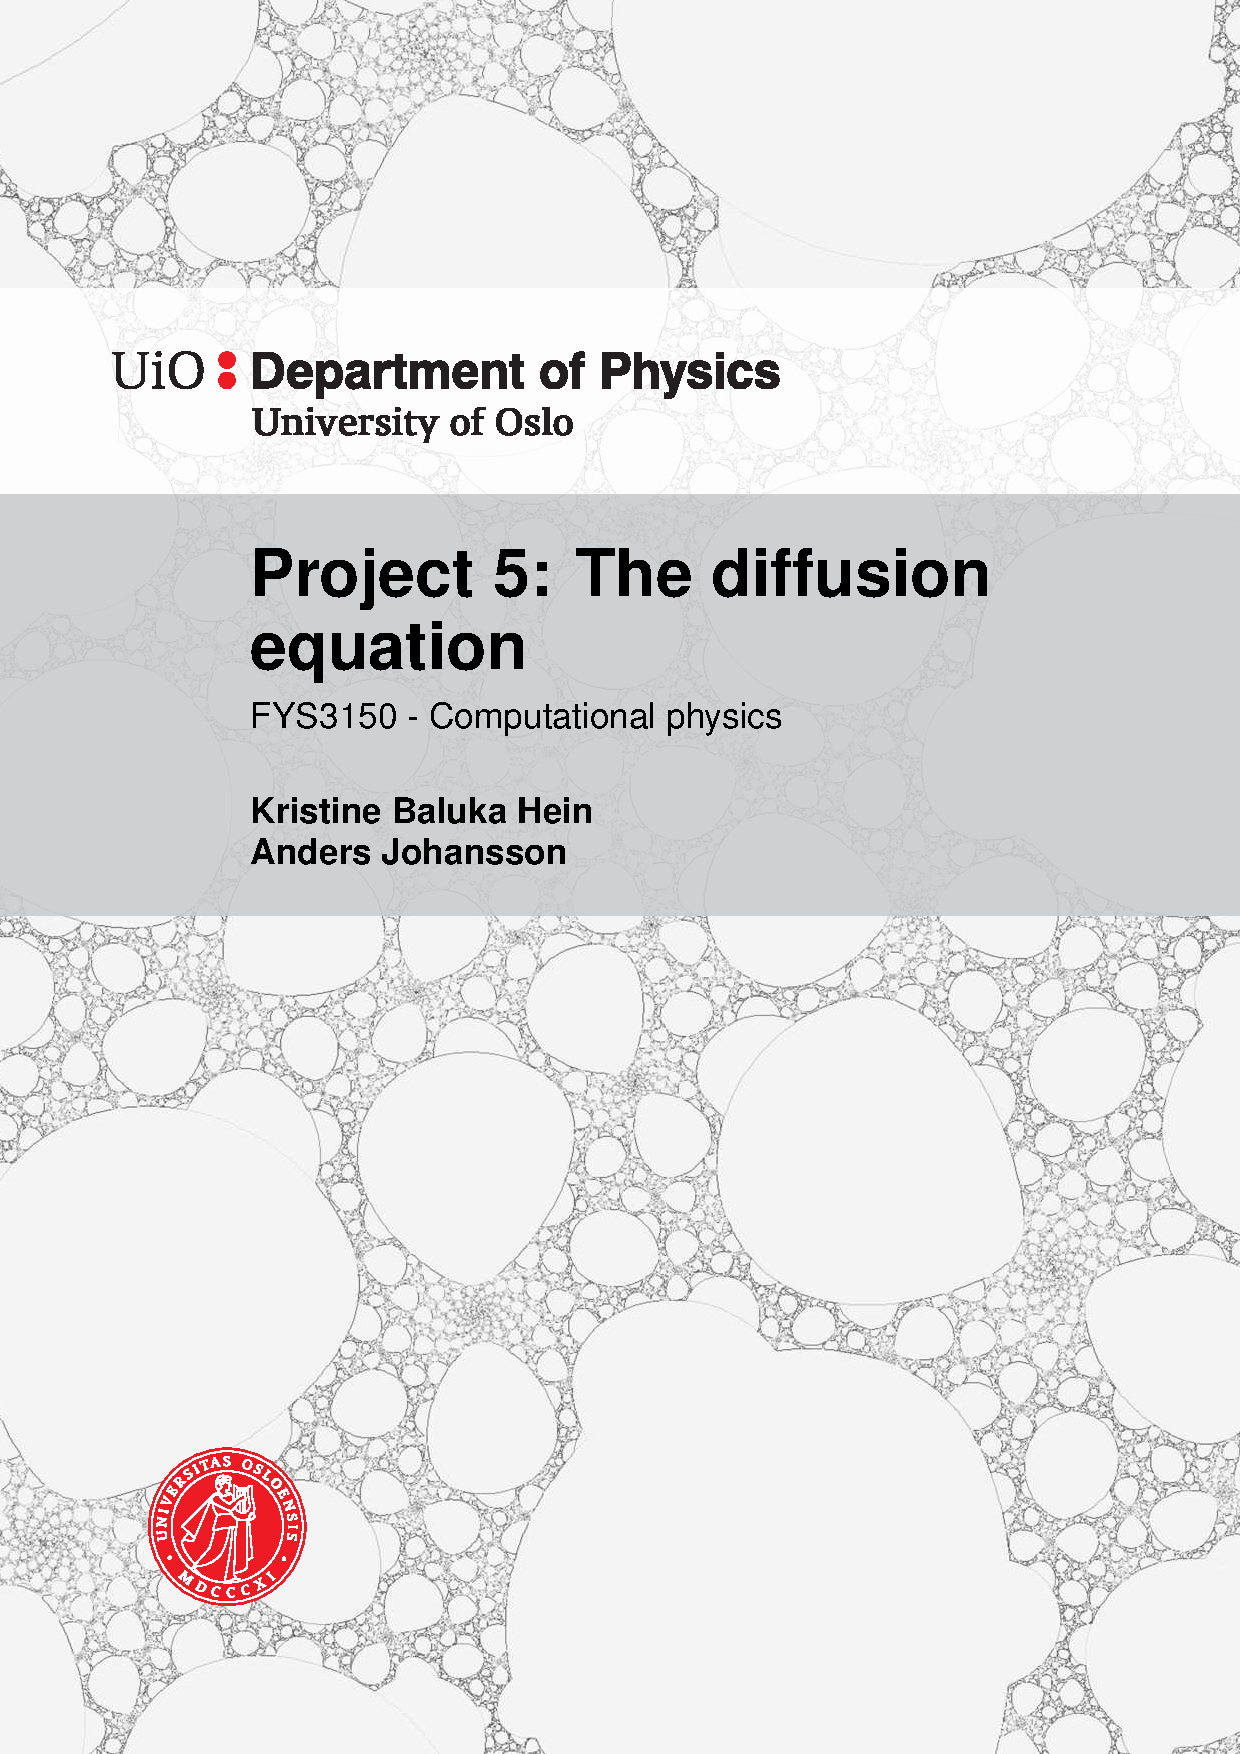
\includepdf{forside.pdf}
%\maketitle
\pagestyle{fancy}
\tableofcontents

\clearpage
\begin{abstract}
In this report we have presented three different numerical methods to solve the diffusion equation in one dimension. The three presented methods are the Forward Euler, Backward Euler and Crank-Nicolson scheme. We will see that the we have to use the Forward Euler with precaution as it may give erroneous results. However, this will not be the case for the Backward Euler and Crank-Nicolson. We will also see that the Crank-Nicolson gives us the most accurate results.
Furthermore, we will look at a similar solver for solving the equation in two dimensions using the very same idea as for the Forward Euler in one dimension.
\end{abstract}

\section{Introduction}
Partial differential equations are important in many fields of science. These equations can describe the behaviour of many natural phenomenas such as waves of sound or sea, the flow of a liquid, growth of a population or diffusion, which is the phenomenon studied in this report. Diffusion is an important process which we find everywhere around us, from water softening spaghetti by diffusing into it to the random motion of viruses on the hunt for fresh cells to destroy.

Partial differential equations are often solved numerically since an analytical solution is difficult, or even impossible to find. An example of the latter is the Navier-Stokes equation to model the flow of a viscous fluid when not certain assumptions to simplify the equations have been made.

In this report we will focus on how we can numerically solve the diffusion equation on a dimensionless form, which is written as
\begin{equation}\label{eq:diffusion}
\begin{aligned}
\pdv{u}{t} = \nabla^2 u
\end{aligned}
\end{equation}
After deriving Fick's laws of diffusion, we derive and analyse methods for solving the equation in both one and two dimensions. Only the explicit Forward Euler scheme is used in two dimensions, while the one-dimensional equation is also solved with the implicit Backward Euler and Crank-Nicolson schemes. In one dimension, von Neumann stability analysis is used to find criteria which guarantee the stability of the methods. Analytical solutions are found in both cases for verification of the methods and error analysis.


\clearpage
%   __           _ _    _
%  / _|_   _ ___(_) | _| | __
% | |_| | | / __| | |/ / |/ /
% |  _| |_| \__ \ |   <|   <
% |_|  \__, |___/_|_|\_\_|\_\
%      |___/
\section{Physical theory of diffusion}\label{sec:physics}
Diffusion is simply the net movement of particles as a result of a random walk, and can be modelled as each atom constantly making a jump in a random  direction. It may seem a little counterintuitive that random motion can lead to a net flow, but consider that if there are \(10\) particles to the left, of which half move to the right, and \(100\) particles on the right, of which half move to the left, the net result is \(45\) particles moving to the left. The opposite of diffusion is drift, where the net motion is a result of an external driving force, for example an electric field.

The two most important equations in diffusion are Fick's laws, which, in one dimension, state that
\[
J = -D\pdv{C}{x} \qquad \qquad \pdv{C}{t} = D\pdv[2]{C}{x}
\]
where \(D\) is the diffusion coefficient, \(J\) the flux, i.e. the number of particles moving per area, and \(C\) the concentration, i.e. the number of particles per volume. Fick's second law, which is also simply called the diffusion equation, is the partial differential equation which is solved numerically on a dimensionless form in this project.


%  _____ _      _    _        __ _          _
% |  ___(_) ___| | _( )___   / _(_)_ __ ___| |_
% | |_  | |/ __| |/ /// __| | |_| | '__/ __| __|
% |  _| | | (__|   <  \__ \ |  _| | |  \__ \ |_
% |_|   |_|\___|_|\_\ |___/ |_| |_|_|  |___/\__|
\subsection{Derivation of Fick's first law in one dimension}
\begin{figure}[H]
    \centering
    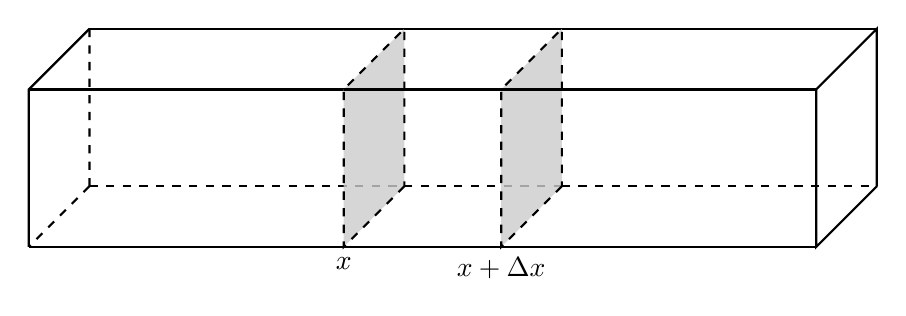
\begin{tikzpicture}[thick]
        \draw (0,0,2) -- (0,2,2) -- (0,2,0);
        \draw[dashed] (0,0,0) -- (0,0,2) (0,2,0) -- (0,0,0);
        \draw[dashed] (0,0,0) -- (4,0,0);
        \draw (0,0,2) -- (4,0,2);
        \draw (0,2,2) -- (4,2,2);
        \draw (0,2,0) -- (4,2,0);
        \fill[black!20!white,opacity=0.8] (4,0,0) -- (4,0,2) node[anchor=north] {\(x\)} -- (4,2,2) -- (4,2,0) -- (4,0,0);
        \draw[dashed] (4,0,0) -- (4,0,2) node[anchor=north] {\(x\)} -- (4,2,2) -- (4,2,0) -- (4,0,0);
        \draw[dashed] (6,0,0) -- (4,0,0);
        \draw (6,0,2) -- (4,0,2);
        \draw (6,2,2) -- (4,2,2);
        \draw (6,2,0) -- (4,2,0);
        \fill[black!20!white,opacity=0.8] (6,0,0) -- (6,0,2) -- (6,2,2) -- (6,2,0) -- (6,0,0);

        \draw[dashed] (6,0,0) -- (6,0,2) node[anchor=north] {\(x+\Delta x\)} -- (6,2,2) -- (6,2,0) -- (6,0,0);
        \draw[dashed] (6,0,0) -- (10,0,0);
        \draw (6,0,2) -- (10,0,2);
        \draw (6,2,2) -- (10,2,2);
        \draw (6,2,0) -- (10,2,0);
        \draw (10,0,0) -- (10,0,2) -- (10,2,2) -- (10,2,0) -- (10,0,0);
    \end{tikzpicture}
    \caption{Sketch of the infinitesimal volume element used in the derivation of Fick's laws in one dimension. Drawn in TikZ.}\label{fig:fick}
\end{figure}

As stated above, diffusion is the process of random walk. In one dimension, this means that each particle will have a \(\SI{50}{\percent}\) probability of moving one step to the left, and a \(\SI{50}{\percent}\) probability of moving one step to the right. As such, the net movement of particles to the right between \(x\) and \(x+\Delta x\) equals half the particles at point \(x\) minus half the particles at point \(x+\Delta x\). Since the flux is the movement of particles per cross-section area \(A\) (marked with grey in the figure) per time interval \(\Delta t\), this can be formulated mathematically as
\[
    J = -\frac{N(x+\Delta x, t) - N(x,t)}{2A\Delta t}
\]
Multiplying by \(\qty(\Delta x)^2\) in both the numerator and the denominator, and factoring out the \(\Delta t\), we get
\[
    J = -\frac{\qty(\Delta x)^2}{2\Delta t}\qty(\frac{N(x+\Delta x,t) - N(x,t)}{A\Delta x\cdot\Delta x})
\]
Since \(A\Delta x\) is a small volume element, \(C=N/\qty(A\Delta x)\):
\[
    J = -\frac{\qty(\Delta x)^2}{2\Delta t} \qty(\frac{C(x+\Delta x,t) - C(x,t)}{\Delta x})
\]
Defining \(D=\qty(\Delta x)^2/2\Delta t\) and letting \(\Delta x\to0\) gives Fick's first law:
\[
    J = -D\pdv{C}{x}
\]


%  _____ _      _    _                                    _
% |  ___(_) ___| | _( )___   ___  ___  ___ ___  _ __   __| |
% | |_  | |/ __| |/ /// __| / __|/ _ \/ __/ _ \| '_ \ / _` |
% |  _| | | (__|   <  \__ \ \__ \  __/ (_| (_) | | | | (_| |
% |_|   |_|\___|_|\_\ |___/ |___/\___|\___\___/|_| |_|\__,_|
\subsection{Derivation of Fick's second law in one dimension}
The derivation of Fick's second law is based on finding two different expressions for the change in the number of particles between \(x\) and \(x+\Delta x\), setting them equal to each other and inserting Fick's first law into the result.

To find the change in number of particles between the two grey surfaces in \vref{fig:fick} over a time interval \(\Delta t\), remember that the flux is defined as the number of particles passing per cross-section \(A\) per time interval \(\Delta t\). Therefore, the number of particles moving out of the volume between \(x\) and \(x+\Delta x\) in a time interval \(\Delta t\) is \(J(x+\Delta x,t)A\Delta t\), while the number of particles moving into the volume is \(J(x,t)A\Delta t\). Thus, the net change in the number of particles between \(x\) and \(\Delta x\) can be written as
\[
    \qty(J(x,t) - J(x + \Delta x,t))A\Delta t = -\qty(J(x+\Delta x,t) - J(x,t))A\Delta t
\]
On the other hand, this change in the number of particles must also equal the change in concentration \(C(x,t+\Delta t) - C(x,t)\), multiplied with the volume, \(A\Delta x\). Since these two methods of calculating the change in the number of particles must give the same result, the following equation must hold:
\begin{alignat*}{2}
    -\qty(J(x+\Delta x,t) - J(x,t))A\Delta t &= \qty(C(x,t+\Delta t) - C(x,t)) A\Delta x\\
    \frac{J(x+\Delta x,t) - J(x,t)}{\Delta x} &= -\frac{C(x,t+\Delta t) - C(x,t)}{\Delta t}
\end{alignat*}
Letting \(\Delta x\to0\) and \(\Delta t\to0\), we get the so-called continuity equation:
\[
    \pdv{J}{x} = -\pdv{C}{t}
\]
Inserting Fick's first law for \(J\) on the left hand side, Fick's second law appears:
\begin{alignat*}{2}
    \pdv{x}\qty(-D\pdv{C}{x}) &= -\pdv{C}{t}\\
    D\pdv[2]{C}{x} &= \pdv{C}{t}
\end{alignat*}


%      _                 _             _        _
%  ___| |_ ___  __ _  __| |_   _   ___| |_ __ _| |_ ___
% / __| __/ _ \/ _` |/ _` | | | | / __| __/ _` | __/ _ \
% \__ \ ||  __/ (_| | (_| | |_| | \__ \ || (_| | ||  __/
% |___/\__\___|\__,_|\__,_|\__, | |___/\__\__,_|\__\___|
%                          |___/
\subsection{Steady state}\label{steadystate}
When \(t\to\infty\), the system will reach a steady state where the concentration at each point does not change with time. A different formulation is that for each volume element, the number of particles entering must be the same as the number of particles leaving, which means that the flux must be the same at all points. Using Fick's first law, this can be formulated as
\[
\text{constant} = J = -D\pdv{C}{x}
\]
which means that the concentration must be a linear function of \(x\). This is a test which both the analytical and the numerical solutions must pass.


%  _       _ _   _       _     _                           _
% (_)_ __ (_) |_(_) __ _| |   | |__   ___  _   _ _ __   __| | __ _ _ __ _   _
% | | '_ \| | __| |/ _` | |   | '_ \ / _ \| | | | '_ \ / _` |/ _` | '__| | | |
% | | | | | | |_| | (_| | |_  | |_) | (_) | |_| | | | | (_| | (_| | |  | |_| |
% |_|_| |_|_|\__|_|\__,_|_( ) |_.__/ \___/ \__,_|_| |_|\__,_|\__,_|_|   \__, |
%                         |/                                            |___/
\subsection{Initial and boundary conditions}
We will study a situation with a constant source at \(x=L\) and a drain at \(x=0\), with the system initially containing \(0\) particles everywhere but at the source. In the dimensionless form, this can be formulated as
\begin{alignat*}{6}
u(x,0) &= 0\qquad & x&\in\left[0,1\right)\\
u(0,t) &= 0\qquad & t&\in\mathbb{R}\\
u(L,t) &= 1\qquad & t&\in\mathbb{R}
\end{alignat*}


%                       _ _
%   ___  _ __   ___  __| (_)_ __ ___
%  / _ \| '_ \ / _ \/ _` | | '_ ` _ \
% | (_) | | | |  __/ (_| | | | | | | |
%  \___/|_| |_|\___|\__,_|_|_| |_| |_|
\clearpage
\section{Mathematical theory in one dimension}
Before we can begin our analysis on how it is possible to numerically solve the diffusion equation, we will first take a look at the analytical solution. This analytical solution can be used in von Neumann analysis to find requirements for the numerical parameters to ensure that a reasonable solution is found.
\subsection{Analytical solution of the diffusion equation}\label{sec:analyticalOneDim}
Consider the diffusion equation with the given boundaries:
\begin{equation}\label{eq:problem}
\begin{aligned}
\pdv[2]{u(x,t)}{x} &= \pdv{u(x,t)}{t} &\: t>0, \:\:x\in[0,L] \\
u(x,0) &= g(x)  &0 < x < L\\
u(0,t) &=  a & a \in \mathbb{R},  t>0 \\
u(L,t) &= b &b \in \mathbb{R}, t>0
\end{aligned}
\end{equation}
As will become clear later, life is much easier when \(a\) and \(b\) are both zero. As such, we introduce a new function
\[
v(x,t) = u(x,t) + w(x,t)
\]
where \(u\) is a solution of \ref{eq:problem} and the following also holds:
\begin{equation}\label{eq:dummy}
    \begin{aligned}
        \pdv[2]{v(x,t)}{x} &= \pdv{v(x,t)}{t} &\: t>0, \:\:x\in[0,L] \\
        v(x,0) &= f(x)  &0 < x < L\\
        v(0,t) &=  0 &  t>0 \\
        v(L,t) &= 0 & t>0
    \end{aligned}
\end{equation}
When introducing \(v(x,t)\), a new problem arises: What does \(w(x,t)\) actually look like? Inserting the definition of \(v\) into \ref{eq:dummy} gives
\begin{alignat*}{2}
    \pdv[2]{v(x,t)}{x} &= \pdv{v(x,t)}{t}  \\
    \pdv[2]{u(x,t)}{x} + \pdv[2]{w(x,t)}{x} &= \pdv{u(x,t)}{t} + \pdv{w(x,t)}{t}
\end{alignat*}
The assumption that \(u\) is a solution to the original problem, which means that
\[
    \pdv[2]{u(x,t)}{x} = \pdv{u(x,t)}{t}
\]
As a result, \ref{eq:dummy} will hold if
\begin{equation} \label{eq:dummy1}
    \pdv[2]{w(x,t)}{x} = 0 = \pdv{w(x,t)}{t}
\end{equation}
These two equalities are separately fulfilled if
\begin{alignat*}{2}
	\pdv[2]{w(x,t)}{x}  &= 0\\
	\pdv{w(x,t)}{x} &= A + h_1(t)\\
	w(x,t) &= Ax +xh_1(t) + B + h_2(t) \eqtag{eq:wX}
\shortintertext{and}
    \pdv{w(x,t)}{t} &= 0\\
    w(x,t) &= C + h_3(x)\eqtag{eq:wT}
\intertext{Combining these two requirements for \(w\), we see that it must be on the form}
    w(x,t) &= w(x) = Ax + D
\end{alignat*}
because there is no dependence of \(t\) in \vref{eq:wT}.

We have now found a possible form for \(w\). However, the values of \(A\) and \(D\) still need to be determined. This can be done by looking at the boundary conditions for \(v\) at \(x = 0 \) and \(x = L\) and using the assumption that \(u\) fulfills the boundary conditions of \ref{eq:problem}, i.e. \(u(0,t)=a\):
\[
    0 = v(0,t) = u(0,t) + w(x=0) = a+D
\]
which implies \(D = -a\). Similarly, the boundary at \(x=L\) gives
\[
    0 = v(L,t) = u(L,t) + w(x=L) = b+AL-a \implies A = \frac{a-b}{L}
\]
In conclusion, we have
\[
    w(x) = \frac{a-b}{L}x - a
\]
As the expression of \(w\) has been found, we have also found \(f(x)\) in \vref{eq:dummy}:
\begin{align*}
	v(x,0) &= u(x,0) + w(x) \\
	&= g(x)+w(x) \\
	&=f(x)
\end{align*}
Having set up the problem properly, we are now ready to solve for \(v(x,t)\). To do so, we make the assumption that \(v\) is separable, i.e. it can be written as
\[
    v(x,t) = F(x)G(t)
\]
which means that
\begin{alignat*}{2}
    \pdv[2]{v(x,t)}{x} &= \pdv{v(x,t)}{t}\\
    F''(x)G(t) &= F(x)G'(t)\\
    \frac{F''(x)}{F(x)} &= \frac{G'(t)}{G(t)}
\end{alignat*}
As the two sides of the last equation depend on different variables which can be varied independently, both sides must equal some constant \(-\lambda\):
\[
    \frac{F''(x)}{F(x)} = \frac{G'(t)}{G(t)} = -\lambda\eqtag{eq:ration}
\]
Solving for \(F\) we get
\[
	F'' = -\lambda F
\]
with a general solution
\[
    F(x) = c_1\cos(x\sqrt{\lambda} ) + c_2\sin(x\sqrt{\lambda})
\]
To find the constants \(c_1\) and \(c_2\), we will use the boundaries for \(v(x,t)\) at \(x = 0\) and \(x = L\). The advantage of having the boundary conditions equal to zero now becomes apparent, as this implies
\begin{alignat*}{8}
    0 &= v(0,t) &= F(0)G(t) \implies F(0) &= 0
    \shortintertext{and}
    0 &= v(L,t) &= F(L)G(t) \implies F(L) &= 0
\end{alignat*}
Since \(\sin(0)=0\neq\cos(0)\), we must have that
\begin{alignat*}{2}
    0 &= c_1
    \shortintertext{and}
    0 &=  c_2\sin(L\sqrt{\lambda})
\intertext{Of course, \(c_2\) could also be set to \(0\), but this is the trivial solution which is of no interest. Therefore, we must have}
    0 &= \sin(L\sqrt{\lambda})
\end{alignat*}
Since sine is zero for every integer multiple of \(\pi\), we have that
\begin{alignat*}{2}
    L\sqrt{\lambda} &= k\pi \quad k\in \mathbb{N}\\
    \lambda &= \qty(\frac{k \pi}{L})^2
\end{alignat*}
In conclusion, the following is a solution for all \(k\in\mathbb{N}\):
\[
    F_k(x) = c_k\sin(x\frac{k \pi}{L})
\]
Similarly, \ref{eq:ration} implies that
\[
    G_k'(t) = -\lambda_k G_k(t) \implies
    G_k(t) = C_k\exp{-\qty(\frac{k \pi}{L})^2t}
\]
For simplicity, \(C_k\) can be absorbed into \(c_k\).

We are now close to an expression for \(v\):
\[
    v_k(x,t) = c_k\exp{-\qty(\frac{k \pi}{L})^2t}\sin(x\frac{k \pi}{L})
\]
What remains is to find \(c_k\). The final, unused piece of information is the initial condition, i.e. \(v(x,0)\). Inserting \(t=0\) in the equation above makes the exponential \(1\), i.e.
\[
    f(x) = c_k\sin(x\frac{k \pi}{L})
\]
Multiplying  the equation above by \(\sin(x\frac{k \pi}{L})\), integrating both sides and using the orthogonality of sine (note that this sine is \(L\)-periodic), gives us
\begin{align*}
    \int_0^Lf(x)\sin(x\frac{k \pi}{L})\dd{x} &= c_k\frac{L}{2} \\
    \frac{2}{L}\int_0^Lf(x)\sin(x\frac{k \pi}{L})\dd{x} &= c_k
\end{align*}
However, we are not looking for one particular solution of \ref{eq:dummy}, but for all solutions. From the principle of superposition, every particular solution contributes to another solution. Specifically, this means that
\[
    v(x,t) = \sum_{k=1}^\infty v_k(x,t)
\]

Remember now the original ansatz
\[
    v(x,t) = u(x,t) + w(x,t)
\]
As \(v\) and \(w\) have now been determined, \(u\) can be found through a reorganisation:
\begin{align*}
    u(x,t) &= v(x,t)- w(x,t) \\
    &=  \sum_{k=1}^\infty v_k(x,t) - w(x) \\
    &=\sum_{k=1}^\infty c_k\exp{-\qty(\frac{k \pi}{L})^2t}\sin(x\frac{k \pi}{L})  -\qty(\frac{a-b}{L}x - a)
\end{align*}
with
\[
    c_k = \frac{2}{L}\int_0^Lf(x)\sin(x\frac{k \pi}{L})\dd{x}
\]
\hfill \\
For our case, that is \vref{eq:diffusion}, we have that \(a = 0\), \(b = 1\), \(g(x) = 0\) and \(L = 1\). Inserting this into the solution of \vref{eq:dummy} gives us
\begin{equation}\label{eq:analyticalSolution}
	u(x,t) = \sum_{k=1}^\infty c_k\exp{-(k\pi)^2t}\sin(xk\pi)  + x
\end{equation}
with
\begin{align*}
    c_k &= 2\int_0^1(0-x)\cdot\sin(xk\pi)\dd{x}
    = - \frac{2}{k\pi}\qty[\frac{\sin(k\pi x)}{k\pi} - x\cos(k\pi x)]_0^1
    = \frac{2(-1)^{k+2}}{k\pi}
    =  \frac{2(-1)^k}{k\pi}
\end{align*}


%      _ _                   _   _           _   _
%   __| (_)___  ___ _ __ ___| |_(_)___  __ _| |_(_) ___  _ __
%  / _` | / __|/ __| '__/ _ \ __| / __|/ _` | __| |/ _ \| '_ \
% | (_| | \__ \ (__| | |  __/ |_| \__ \ (_| | |_| | (_) | | | |
%  \__,_|_|___/\___|_|  \___|\__|_|___/\__,_|\__|_|\___/|_| |_|
\subsection{Discretisation}

\todo[inline]{Forslag: Since the solution is an infinite series of Fourier coefficients, it cannot be computed directly numerically. Therefore, it must be discretised.}

For the diffusion equation to be numerically solvable, it must be discretised.

This is done in the standard way: Discretise \(x\) as \(x_0,x_1,\dots,x_n\) with \(\Delta x=\qty(x_n-x_0)/n\), and \(t\) as \(t_0,t_1,\dots,t_m\) with \(\Delta t = \qty(t_m-t_0)/m\). The function itself is also discretised, with the notation \(u_{i,j} \approx u(x_i,t_j)\).

We will now take a look into how we can numerically approximate the given problem. As there exist many different approaches, we have chosen to look at three different methods, namely Forward Euler, Backward Euler and Crank-Nicolson. The difference between Forward Euler and Backward Euler is how the time derivative is approximated, as the Crank-Nicolson method is a combination of both.



%  _____                                _   _____      _
% |  ___|__  _ ____      ____ _ _ __ __| | | ____|   _| | ___ _ __
% | |_ / _ \| '__\ \ /\ / / _` | '__/ _` | |  _|| | | | |/ _ \ '__|
% |  _| (_) | |   \ V  V / (_| | | | (_| | | |__| |_| | |  __/ |
% |_|  \___/|_|    \_/\_/ \__,_|_|  \__,_| |_____\__,_|_|\___|_|
%
\subsection{Forward Euler}
Forward Euler is the simplest and most intuitive algorithm implemented in this report. As we will see later, this simplicity in both idea and implementation comes at a cost, as the Forward Euler scheme is the only algorithm which sets requirements for the values of \(\Delta x\) and \(\Delta t\) to even give a reasonable solution.


\subsubsection{Derivation and error analysis}\label{sec:ForwardEulerDerivation}
The Forward Euler scheme is an explicit scheme based on Taylor polynomials. To find an approximation to the time derivative of \(u\) at point \((x_i,t_j)\), a first order Taylor polynomial around \(x_i,t_j\) is used to calculate \(u(x_i,t_{j+1})\):
\[
    u_{i,j+1} = u_{i,j} + h\pdv{u_{i,j}}{t} + \frac{1}{2}\qty(\Delta t)^2\pdv[2]{u(x_i,\tilde{t})}{t}
    \implies \pdv{u_{i,j}}{t} = \frac{u_{i,j+1}-u_{i,j}}{\Delta t} + \frac{1}{2}\Delta t\pdv[2]{u(x_i,\tilde{t})}{t}\eqtag{asymmnewton}
\]
where \(\tilde{t}\in(t_j,t_{j+1})\) and the last term is the truncation error, which is proportional to \(\Delta t\).

Similarly, the three point approximation to the second derivative (derived in \autocite{oblig1}) with its error is used to approximate the second derivative of \(u\) at point \((x_i,t_j)\) with respect to position:
\[
    \pdv[2]{u_{i,j}}{x} = \frac{u_{i+1,j} + u_{i-1,j} - 2u_{i,j}}{\qty(\Delta x)^2} - \frac{1}{12}\qty(\Delta x)^2\pdv[4]{u(\tilde{x},t_j)}{x}\eqtag{andrederivert}
\]
where the last term is the truncation error, which for this approximation is proportional to \(\qty(\Delta x)^2\). As shown in \autocite{oblig1}, the error term actually consists of two terms, one with \(\tilde{x}_1\in\qty(x_{i-1},x_i)\) and one with \(\tilde{x}_2\in\qty(x_i,x_{i+1})\), but this can be approximated with \(\tilde{x}\in(x_{i-1},x_{i+1})\).

Inserting these two expressions into the diffusion equation gives
\[
    \frac{u_{i,j+1}-u_{i,j}}{\Delta t} + \frac{1}{2}\Delta t\pdv[2]{u(x_i,\tilde{t})}{t}
    = \frac{u_{i+1,j} + u_{i-1,j} - 2u_{i,j}}{\qty(\Delta x)^2} - \frac{1}{12}\qty(\Delta x)^2\pdv[4]{u(\tilde{x},t_j)}{x}
\]
The goal is to find the value of \(u\) at the next time step, i.e. \(u_{i,j+1}\). Multiplying by \(\Delta t\) on both sides of the equation and moving one term to the right, we get
\begin{alignat*}{2}
    u_{i,j+1} &=&& u_{i,j} + \frac{\Delta t}{\qty(\Delta x)^2}\qty(u_{i+1,j} + u_{i-1,j}-2u_{i,j})\\
    &&&+ \frac{1}{2}\qty(\Delta t)^2\pdv[2]{u(x_i,\tilde{t})}{t} - \Delta t\cdot\frac{1}{12}\qty(\Delta x)^2\pdv[4]{u(\tilde{x},t_j)}{x}
    \intertext{The quantity \(\Delta t/\qty(\Delta x)^2\) can be defined as \(\alpha\), which, with a slight reorganisation yields the final expression}
    u_{i,j+1} &=&& \qty(1-2\alpha)u_{i,j} + \alpha\qty(u_{i+1,j}+u_{i-1,j})\\
    &&& +  \frac{1}{2}\qty(\Delta t)^2\pdv[2]{u(x_i,\tilde{t})}{t} - \Delta t\cdot\frac{1}{12}\qty(\Delta x)^2\pdv[4]{u(\tilde{x},t_j)}{x}
\end{alignat*}
The two error terms are proportional to \(\qty(\Delta t)^2\) and \(\Delta t\cdot \qty(\Delta x)^2\). As per usual, the global error is one order lower, as the error is accumulated. This gives one error term proportional to \(\Delta t\) and one proportional to \(\qty(\Delta x)^2\). The order of \(\qty(\Delta x)\) is not reduced, as this error is not accumulated. If we truncate the errors in \(u_{i,j}\) , we get the numerical approximation of \(u(x_i,t_{j+1})\) to be
\begin{equation}\label{eq:forwardEuler}
u_{i,j+1} = \qty(1-2\alpha)u_{i,j} + \alpha\qty(u_{i+1,j}+u_{i-1,j})
\end{equation}


%                     _   _
% __   _____  _ __   | \ | | ___ _   _ _ __ ___   __ _ _ __  _ __
% \ \ / / _ \| '_ \  |  \| |/ _ \ | | | '_ ` _ \ / _` | '_ \| '_ \
%  \ V / (_) | | | | | |\  |  __/ |_| | | | | | | (_| | | | | | | |
%   \_/ \___/|_| |_| |_| \_|\___|\__,_|_| |_| |_|\__,_|_| |_|_| |_|

\subsubsection{The idea behind von Neumann stability analysis}\label{sec:ideaNeumann}
As we now have set up the algorithm using Forward Euler to approximate the derivatives, we might ask ourselves whether this method gives us stable results. This is an important question, since it may happen that the numerical errors propagate in such a manner that it will corrupt the final results. To see whether this is the case, we will use the method of von Neumann to study the stability of the Forward Euler scheme, as well as the Backward Euler and Crank-Nicolson schemes.


The problem of approximating \(u(x,t)\) is to sufficiently approximate the infinite series given in \vref{eq:analyticalSolution} and the exact value of the \(c_k\)s. Since \( x\) does not include infinity and therefore can be computed directly, we can assume that \(x\) will not contribute to the propagation of error. Therefore, we must look at the stability when calculating \( \sum_{k=1}^\infty c_ke^{-(k\pi)^2t}\sin(xk\pi) \), i.e the solution of \(v(x,t)\) to make sure it will not blow up the solution of \(u(x,t)\).

If we proceed in the similar manner as for finding the analytical solution and making the ansatz that
\begin{equation}\label{eq:discreteAnsatz}
    v_{k_{i,j}} = F_k(x_i)G_k(t_j)
\end{equation}

and introducing \(D_x^2\) and \(D_t\) as the numerical approximations of the spatial and time derivatives respectively, we get that
\[
    G(t_j)\:\qty(D_x^2F_k(x))_i = F(x_i)\:\qty(D_tG(t))_j
\]
where \(\qty(D_x^2F_k(x))_i\) and \(\qty(D_tG(t))_j\) means that we are taking the derivative around the \(i\)-th and \(j\)-th step respectively.
From what we found above, we have that
\begin{equation}\label{eq:discreteRatios}
    \frac{\qty(D_x^2F_k(x))_i }{ F(x_i)} = \frac{\qty(D_tG_k(t))_j}{G_k(t_j)} = -\mu_{k_{i,j}}
\end{equation}
The second derivative of \(x\) is approximated using the second order central difference equation, i.e \vref{andrederivert}.
From the analytical solution, we can assume that \(F(x_i) = \sin(k \pi x_i)\). This gives
\begin{align*}
    \qty(D_x^2F_k(x))_i &= -\mu_{k_{i,j}}F(x_i) \\
    \frac{F(x_{i-1}) -2F(x_i) + F(x_{i+1}) }{\Delta t^2} &= -\mu_{k_{i,j}}F(x_i) \\
    \sin(k\pi x_{i-1}) -2\sin(k\pi x_i) + \sin(k \pi x_{i+1}) &= -\Delta t^2\mu_{k_{i,j}}\sin(k \pi x_i)
\end{align*}
Using the trigonometric identities
\[
    \sin(k\pi x_{i-1}) + \sin(k\pi x_{i+1}) = 2\cos(k\pi \Delta t)\sin(k\pi x_i)
\]
we get
\[
    \sin(k\pi x_i)(2\cos(k\pi \Delta t) - 2) = -\Delta t^2\mu_{k_{i,j}}\sin(k \pi x_i)
\]
The factor \(\sin(k\pi x_i) \) can never be zero, as the derivative is taken at points in \((0,1) \) since the boundary values are known. The eigenvalue \(\mu_{k_{i,j}}\) of the approximation of the second derivative with respect to \(x \), \( D_x^2 \), is therefore
\begin{equation}\label{eq:eigenvalue1}
    \frac{-2\qty(\cos(k\pi \Delta t) - 1)}{\Delta t^2} =\mu_{k_{i,j}}
\end{equation}
Furthermore, we have the identity
\begin{align*}
    \cos(x) &= \cos^2\qty(\frac{x}{2}) - \sin^2\qty(\frac{x}{2}) \\
    &= 1- 2\sin^2\qty(\frac{x}{2}) \\
    1-\cos(x) &= 2\sin^2\qty(\frac{x}{2})
\end{align*}
and by inserting this into \vref{eq:eigenvalue1}, we get the following eigenvalue
\begin{equation} \label{eq:mu}
    \frac{4\sin^2\qty(\frac{k\pi \Delta t}{2})}{\Delta t^2} =\mu_{k_{i,j}} = \mu_k
\end{equation}

Now we have proven that assuming \(F_k(x_i) = \sin(k\pi x_i)\) is not a such bad idea, as the guess is reasonable compared to the analytical solution and no other contradictions have arised.

We see from the analytical solution that the function of time, \(G_k(t) = \exp{-\lambda_k t}\) is decreasing for increasing values of \(t\), meaning that the discrete functions of time should behave in equivalent manner.

Therefore the computed function of time, \(G_k(t_j)\), must hold the following constraints
\[
    G_k(t_{0}) = 1 \quad \text{ and }\quad \abs{\frac{G_k(t_{j+1}) } {G_k(t_j) } }\leq 1 \:\:\text{ for } j = 0, \dots,m-1
\]

We include that the fraction could be equal to one as it may happen that we could be very close to the likely state, that is when \(t \to \infty \)  , giving us \( G_k(t_{j+1}) \approx G_k(t_{j})\).

When the ratio above holds, we have that the solution does not grow for every time step, ensuring that the computed solution is stable for every time step.

Since the expression of \(G_k(t_{j})\) will depend on the choice of numerical scheme, we must do sufficient restrictions for every scheme  such that \(G_k(t_{j})\) does not increase for an increasing time step.



%      _        _     _ _ _ _
%  ___| |_ __ _| |__ (_) (_) |_ _   _
% / __| __/ _` | '_ \| | | | __| | | |
% \__ \ || (_| | |_) | | | | |_| |_| |
% |___/\__\__,_|_.__/|_|_|_|\__|\__, |
%                               |___/
\subsubsection{Stability analysis of Forward Euler}\label{forwardstability}

To approximate the time derivative of Forward Euler, we get the ratios in \ref{eq:discreteRatios} to be
\begin{alignat*}{2}
    \qty(D_tG_k(t))_j &= -G_k(t_j)\mu_k \\
    \frac{G_k(t_{j+1}) - G_k(t_j) }{\Delta t} &= -G_k(t_j)\mu_k \\
    G_k(t_{j+1}) &= -\Delta t G_k(t_j)\mu_k + G_k(t_j) \\
    \frac{G_k(t_{j+1}) }{G_k(t_j)} &= 1-\Delta t \mu_k
\intertext{As discussed in \ref{sec:ideaNeumann}, we must have that}
    \abs{\frac{G_k(t_{j+1}) }{G_k(t_j)}} &\leq 1 \\
    \abs{1-\Delta t \mu_k} &\leq 1\\
    \abs{\Delta t \mu_k} &\leq 2\\
    \abs{\frac{4 \Delta t \sin^2\qty(\frac{k\pi \Delta x}{2})}{\Delta x^2} } &\leq 2 \\
    \abs{\frac{\Delta t \sin^2\qty(\frac{k\pi \Delta x}{2})}{\Delta x^2} } &\leq \frac{1}{2}
\intertext{Since \(\sin^2\qty(\frac{k\pi \Delta x}{2}) \leq 1\) for any \(k\) and \(\Delta x\), this simplifies to}
    \frac{\Delta t}{\Delta x^2} &\leq \frac{1}{2}\eqtag{eq:stabilityForwardEuler}
\end{alignat*}
which is the final criterion for stable results from the Forward Euler scheme.


%  ____             _                           _   _____      _
% | __ )  __ _  ___| | ____      ____ _ _ __ __| | | ____|   _| | ___ _ __
% |  _ \ / _` |/ __| |/ /\ \ /\ / / _` | '__/ _` | |  _|| | | | |/ _ \ '__|
% | |_) | (_| | (__|   <  \ V  V / (_| | | | (_| | | |__| |_| | |  __/ |
% |____/ \__,_|\___|_|\_\  \_/\_/ \__,_|_|  \__,_| |_____\__,_|_|\___|_|
%

\subsection{Backward Euler} \label{sec:backwardEuler}
The idea of Backward Euler is similar to that of Forward Euler, as the only difference lies in how we approximate the time derivative of \(u\). The result, however, is the freedom to choose \(\Delta t\) and \(\Delta x\) as we like and be guaranteed a resonable result.
\subsubsection{Derivation and error analysis}
The time derivative of \(u\) at \((x_i,t_j)\) is once again found through a first order Taylor polynomial around \((x_i,t_j)\), but the Taylor polynomial is now used to approximate \(u_{i,j-1}\), rather than \(u_{i,j+1}\) as in the derivation of the Forward Euler scheme:
\[
    u_{i,j-1} = u_{i,j} - \Delta t\pdv{u_{i,j}}{t} + \frac{1}{2}\qty(\Delta t)^2\pdv[2]{u(x_i,\tilde{t})}{t}
    \implies \pdv{u_{i,j}}{t} = \frac{u_{i,j}-u_{i,j-1}}{\Delta t} + \frac{1}{2}\Delta t\pdv[2]{u(x_i,\tilde{t})}{t}
\]
where \(\tilde{t}\) and the second term are the same as defined in \vref{sec:ForwardEulerDerivation}. The same three-point approximation as in\vref{andrederivert} can be reused to approximate the second derivative with respect to \(x\).

With these approximations, the diffusion equation can be written as
\begin{alignat*}{2}
    \frac{u_{i,j}-u_{i,j-1}}{\Delta t} + \frac{1}{2}\Delta t\pdv[2]{u(x_j,\tilde{t})}{t}
    &=&& \frac{u_{i+1,j}  - 2u_{i,j} + u_{i-1,j}}{\qty(\Delta x)^2} + \frac{1}{12}\qty(\Delta x)^2\pdv[4]{u(\tilde{x},t_j)}{x}  \\
    u_{i,j}-u_{i,j-1} &=&& \alpha(u_{i+1,j}  - 2u_{i,j} + u_{i-1,j})\\
    &&& + \Delta t\cdot \frac{1}{12}\qty(\Delta x)^2\pdv[4]{u(\tilde{x},t_j)}{x}  - \frac{1}{2}\qty(\Delta t)^2\pdv[2]{u(x_j,\tilde{t})}{t}\\
    -\alpha u_{i-1,j} + \qty(1+2\alpha)u_{i,j} - \alpha u_{i+1,j} &=&& u_{i,j-1} + \Delta t\cdot \frac{1}{12}\qty(\Delta x)^2\pdv[4]{u(\tilde{x},t_j)}{x}  - \frac{1}{2}\qty(\Delta t)^2\pdv[2]{u(x_j,\tilde{t})}{t}
\end{alignat*}
In this equation, only the \(u\) on the right hand side is known, while the \(u\)'s on the left side are the ones we are interested in. As it is not possible to find an explicit expression for the quantities of interest, this leads to an implicit scheme. Observe that the error is the same as for the Forward Euler scheme.

To solve the equation above, note that it must hold for all \(i\in\qty[1,n-1]\cap\mathbb{N}\). When ignoring the error terms, we get the following set of equations:
\[
    \begin{array}{ccccccc}
        -\alpha \overbrace{u_{0,j}}^0 &+& (1+2\alpha)u_{1,j} &-& \alpha u_{2,j} &=& u_{1,j-1}\\
        -\alpha u_{1,j} &+& (1+2\alpha)u_{2,j} &-& \alpha u_{3,j} &=& u_{2,j-1}\\
        -\alpha u_{2,j} &+& (1+2\alpha)u_{3,j} &-& \alpha u_{4,j} &=& u_{3,j-1}\\
        \vdots && \vdots && \vdots && \vdots\\
        -\alpha u_{n-3,j} &+& (1+2\alpha)u_{n-2,j} &-& \alpha u_{n-1,j} &=& u_{n-2,j-1}\\
        -\alpha u_{n-2,j} &+& (1+2\alpha)u_{n-1,j} &-& \alpha \underbrace{u_{n,j}}_1 &=& u_{n-1,j-1}\\
    \end{array}
\]
This can then be written on a matrix form:
\[
    \begin{bmatrix}
        1 + 2\alpha & -\alpha & 0 & 0 & 0 & \dots & 0 & 0 & 0 & 0  \\
        -\alpha & 1+2\alpha & -\alpha & 0 & 0 & \dots & 0 & 0 & 0 & 0  \\
        0 & -\alpha & 1+2\alpha & -\alpha & 0 & \dots & 0 & 0 & 0 & 0 \\
        \vdots & \vdots &  \ddots & \ddots & \ddots & \vdots & \vdots & \vdots & \vdots & \vdots\\
        0 & 0 & 0 & 0 & 0 & \dots & -\alpha & 1+2\alpha & - \alpha & 0\\
        0 & 0 & 0 & 0 & 0 & 0 & \dots & -\alpha & 1+2\alpha & - \alpha\\
        0 & 0 & 0 & 0 & 0 & 0 & 0 & \dots & -\alpha & 1+2\alpha\\
    \end{bmatrix}
    \begin{bmatrix}
        u_{1,j}\\
        u_{2,j}\\
        u_{3,j}\\
        \vdots\\
        u_{n-3,j}\\
        u_{n-2,j}\\
        u_{n-1,j}\\
    \end{bmatrix}
    =
    \begin{bmatrix}
        u_{1,j-1}\\
        u_{2,j-1}\\
        u_{3,j-1}\\
        \vdots\\
        u_{n-3,j-1}\\
        u_{n-2,j-1}\\
        u_{n-1,j-1} + \alpha\\
    \end{bmatrix}
\]

This is a simple, linear system with a tridiagonal matrix, for which an efficient solving algorithm was developed and implemented in project 1 \cite{oblig1}.


%      _        _     _ _ _ _
%  ___| |_ __ _| |__ (_) (_) |_ _   _
% / __| __/ _` | '_ \| | | | __| | | |
% \__ \ || (_| | |_) | | | | |_| |_| |
% |___/\__\__,_|_.__/|_|_|_|\__|\__, |
%                               |___/
\subsubsection{Stability analysis}
For this scheme we have that \vref{eq:discreteRatios} for \(G_k(t_j)\) becomes
\begin{align*}
\qty(D_tG_k(t))_j &= -G_k(t_j)\mu_k \\
\frac{G_k(t_j) - G_k(t_{j-1}) }{\Delta t} &= -G_k(t_j)\mu_k \\
-G_k(t_{j-1}) &= -\Delta t G_k(t_j)\mu_k - G_k(t_j) \\
\frac{G_k(t_{j}) }{G_k(t_{j-1})} &= \frac{1}{1+\Delta t \mu_k}
\end{align*}
Since \(1+\Delta t \mu_k \geq 1\) for all \(k,\mu_k,\Delta t\), the fraction is less than one for any choice of \(\mu_k,\Delta t\). This means that the Backward Euler scheme is stable for every choice of \(\Delta x, \Delta t\), so there are no restrictions on the choice of \(\Delta x \text{ and } \Delta t\), as opposed to the case with Forward Euler.


%   ____                 _         _   _ _           _
%  / ___|_ __ __ _ _ __ | | __    | \ | (_) ___ ___ | |___  ___  _ __
% | |   | '__/ _` | '_ \| |/ /____|  \| | |/ __/ _ \| / __|/ _ \| '_ \
% | |___| | | (_| | | | |   <_____| |\  | | (_| (_) | \__ \ (_) | | | |
%  \____|_|  \__,_|_| |_|_|\_\    |_| \_|_|\___\___/|_|___/\___/|_| |_|
%
\subsection{Crank-Nicolson} \label{sec:crankNicolson}
The Crank-Nicolson scheme could be thought of as a combination of the Forward and Backward Euler schemes. We will see that also the Crank-Nicolson scheme is stable for any choice of \(\Delta t \) and \(\Delta x\).
\subsubsection{Derivation and error analysis}
The idea of the Crank-Nicolson algorithm is to use the derivatives at the times \(t_i+\tfrac{1}{2}\Delta t\) rather than at \(t_i\), as the asymmetric Newton quotient used in the derivation of the Forward Euler scheme will now be the symmetric Newton quotient, giving an error proportional to \(\qty(\Delta t)^2\) instead of \(\Delta t\):
\[
    \pdv{u(x_i,t_j+\tfrac{1}{2}\Delta t)}{t} = \frac{u_{i,j+1} - u_{i,j}}{\Delta t} + \frac{\qty(\Delta t)^2}{12}\pdv[3]{u(x_i,\tilde{t})}{t}
\]
with \(\tilde{t}\in\qty(t_j,t_{j+1})\).

The three-point formula is again used to approximate the second derivative with respect to \(x\), but as there is no known value of \(u\) at \(t_j+\tfrac{1}{2}\Delta t\), the second derivative at this point is approximated by the mean of the second derivatives at \(t_{j+1}\) and \(t_j\):
\begin{alignat*}{2}
    \pdv[2]{u(x_i,t_j+\tfrac{1}{2}\Delta t)}{x} &=&& \frac{1}{2}\qty(\frac{u_{i+1,j+1} + u_{i-1,j+1} - 2u_{i,j+1})}{\qty(\Delta x)^2} + \frac{u_{i+1,j} + u_{i-1,j} - 2u_{i,j}}{\qty(\Delta x)^2})\\
    &&&+ \frac{\qty(\Delta x)^2}{24}\qty(\pdv[4]{u(\tilde{x}_1,t_{j+1})}{x} + \pdv[4]{u(\tilde{x}_2,t_j)}{x})
\end{alignat*}
with both \(\tilde{x}_1\) and \(\tilde{x}_2\) in \(\qty(x_{i-1},x_{i+1})\).

Inserting these expressions into the diffusion equation gives
\begin{alignat*}{2}
    \frac{u_{i,j+1} - u_{i,j}}{\Delta t}
    &=&& \frac{1}{2}\qty(\frac{u_{i+1,j+1} + u_{i-1,j+1} - 2u_{i,j+1})}{\qty(\Delta x)^2} + \frac{u_{i+1,j} + u_{i-1,j} - 2u_{i,j}}{\qty(\Delta x)^2})\\
    &&&+ \frac{\qty(\Delta x)^2}{24}\qty(\pdv[4]{u(\tilde{x}_1,t_{j+1})}{x} + \pdv[4]{u(\tilde{x}_2,t_j)}{x}) + \frac{\qty(\Delta t)^2}{12}\pdv[3]{u(x_i,\tilde{t})}{t}
    \intertext{We are interested in the solution at \(t_{j+1}\). Multiplying by \(2\Delta t\) on both sides and reusing \(\alpha=\Delta t/\qty(\Delta x)^2\) gives}
    -\alpha u_{i-1,j+1} + \qty(2+2\alpha)u_{i,j+1} - \alpha u_{i+1,j+1} &=&& \alpha u_{i-1,j} + \qty(2-2\alpha)u_{i,j} + \alpha u_{i+1,j}\\
    &&&+ \Delta t\cdot\frac{\qty(\Delta x)^2}{12}\qty(\pdv[4]{u(\tilde{x}_1,t_{j+1})}{x} + \pdv[4]{u(\tilde{x}_2,t_j)}{x}) + \frac{\qty(\Delta t)^3}{6}\pdv[3]{u(x_i,\tilde{t})}{t}
\end{alignat*}
Since the error is once again accumulated, the global error will have one term proportional to \(\qty(\Delta x)^2\) and one term proportional to \(\qty(\Delta t)^2\). The latter is one order better than both Euler schemes. With no possibility of solving for the next time step explicitly, this scheme is also implicit.


We have therefore the following approximation
\begin{equation*}
-\alpha u_{i-1,j+1} + \qty(2+2\alpha)u_{i,j+1} - \alpha u_{i+1,j+1} = \alpha u_{i-1,j} - \qty(2+2\alpha)u_{i,j} + \alpha u_{i+1,j}
\end{equation*}

Solving the above equation is done exactly the same way as for the Backward Euler scheme: As it must hold for all \(i\in\qty[1,n-1]\cap\mathbb{N}\), a linear set of equations arises, which, with \(\beta=2+2\alpha\) and \(\beta'=2-2\alpha\), can be written on a matrix form as

\[
    \begin{bmatrix}
        \beta & -\alpha & 0 & 0 & 0 & \dots & 0 & 0  \\
        -\alpha & \beta & -\alpha & 0 & 0 & \dots & 0 & 0  \\
        0 & -\alpha & \beta & -\alpha & 0 & \dots & 0 & 0 \\
        \vdots & \vdots &  \ddots & \ddots & \ddots & \vdots & \vdots & \vdots\\
        0 & 0 & 0 & \dots & -\alpha & \beta & - \alpha & 0\\
        0 & 0 & 0 & 0 & \dots & -\alpha & \beta & - \alpha\\
        0 & 0 & 0 & 0 & 0 & \dots & -\alpha & \beta\\
    \end{bmatrix}
    \begin{bmatrix}
        u_{1,j+1}\\
        u_{2,j+1}\\
        u_{3,j+1}\\
        \vdots\\
        u_{n-3,j+1}\\
        u_{n-2,j+1}\\
        u_{n-1,j+1}\\
    \end{bmatrix}
    =
    \begin{bmatrix}
        \beta' u_{1,j} + \alpha u_{2,j}\\
        \alpha u_{n-1,j} + \beta' u_{2,j} + \alpha u_{2,j}\\
        \alpha u_{n-2,j} + \beta' u_{3,j} + \alpha u_{3,j}\\
        \vdots\\
        \alpha u_{n-4,j} + \beta' u_{n-3,j} + \alpha u_{n-2,j}\\
        \alpha u_{n-3,j} + \beta' u_{n-2,j} + \alpha u_{n-1,j}\\
        \alpha u_{n-2,j} + \beta' u_{n-1,j} + 2\alpha\\
    \end{bmatrix}
\]
The matrix is once again tridiagonal, so the solver from project 1 can be reused.


%      _        _     _ _ _ _
%  ___| |_ __ _| |__ (_) (_) |_ _   _
% / __| __/ _` | '_ \| | | | __| | | |
% \__ \ || (_| | |_) | | | | |_| |_| |
% |___/\__\__,_|_.__/|_|_|_|\__|\__, |
%                               |___/
\subsubsection{Stability analysis}
Since the Crank-Nicolson scheme is derived from using the approximation of the second derivative with respect to \(x\) at \(v_k(x_i,t_j)\) and \(v_k(x_i,t_{j+1})\), we can use the ansatz in \vref{eq:discreteAnsatz} and rewrite the scheme in the following matter:
\[
\frac{1}{2}\qty(G_k(t_{j+1})\qty(D_x^2F_k(x) )_i +  G_k(t_j)\qty(D_x^2F_k(x))_i ) = \frac{(F_k(x) )_i }{\Delta t}\qty(G_k(t_{j+1}) - G_k(t_j) )
\]
We found in \vref{sec:ideaNeumann} that \(D_x^2F_k(x))_i = -\mu_kF_k(x_i)\), meaning that we can rewrite the equation above into
\begin{align*}
\frac{1}{2}\qty(G_k(t_{j+1})\qty(D_x^2F_k(x) )_i +  G_k(t_j)\qty(D_x^2F_k(x))_i ) &= \frac{F_k(x_i) }{\Delta t}\qty(G_k(t_{j+1}) - G_k(t_j) ) \\ \hfill \\
\frac{1}{2}\qty(-\mu_kF_k(x_i)G_k(t_{j+1}) -\mu_kF_k(x_i)G_k(t_j))&= \frac{F_k(x_i)}{\Delta t}\qty(G_k(t_{j+1}) - G_k(t_j) )  \\\hfill \\
\frac{-\mu_k}{2}\qty(G_k(t_{j+1}) +G_k(t_j))&= \frac{1}{\Delta t}\qty(G_k(t_{j+1}) - G_k(t_j) )  \\\hfill \\
-\frac{\Delta t\mu_k}{2}G_k(t_{j+1}) -\frac{\Delta t\mu_k}{2} G_k(t_j)&= G_k(t_{j+1}) - G_k(t_j)   \\\hfill \\
G_k(t_j)\qty(1-\frac{\Delta t\mu_k}{2})&= G_k(t_{j+1})\qty(1+\frac{\Delta t\mu_k}{2} )    \\\hfill \\
\frac{1-\frac{\Delta t\mu_k}{2}}{1+\frac{\Delta t\mu_k}{2}}&= \frac{G_k(t_{j+1}) }{G_k(t_j)}
\end{align*}
Since the numerator is always smaller than the denominator, the fraction which we found will always satisfy
\[
\abs{\frac{1-\frac{\Delta t\mu_k}{2}}{1+\frac{\Delta t\mu_k}{2}}} \leq 1
\]
independent of which \( \Delta t, \Delta x\) we choose. This means that the Crank-Nicolson scheme is stable for any choice of step lengths for \(t\) and \(x\).


%  _                           _ _
% | |___      _____         __| (_)_ __ ___
% | __\ \ /\ / / _ \ _____ / _` | | '_ ` _ \
% | |_ \ V  V / (_) |_____| (_| | | | | | | |
%  \__| \_/\_/ \___/       \__,_|_|_| |_| |_|
\clearpage
\section{Mathematical theory in two dimensions}
The derivation of Fick's laws can be generalised to higher dimensions, giving
\[
    \vec{J} = -D\nabla C \qquad\qquad \pdv{C}{t} = D\nabla^2C
\]
Our differential equation can therefore be written in two dimensions as
\begin{equation} \label{eq:twoDim}
\pdv[2]{u}{x} + \pdv[2]{u}{y} = \pdv{u}{t}
\end{equation}

Time and position are again discretised, with the notation \(u_{i,j,k} = u(x_i,y_j,t_k)\). For all simulations, \(\Delta y\) will be set equal to \(\Delta x\).

%                    _       _   _           _
%   __ _ _ __   __ _| |_   _| |_(_) ___ __ _| |
%  / _` | '_ \ / _` | | | | | __| |/ __/ _` | |
% | (_| | | | | (_| | | |_| | |_| | (_| (_| | |
%  \__,_|_| |_|\__,_|_|\__, |\__|_|\___\__,_|_|
%                      |___/
\subsection{Analytical solution in two dimensions}
For the two-dimensional case, we have chosen to look at a specific set of initial and boundary conditions which make the analytical solution much easier. This analytical solution will later be used to verify that the numerical solver gives acceptably accurate results.

So, consider \vref{eq:twoDim} with the following boundaries over a spatial domain of size \(L \times L\):
\begin{equation} \label{eq:twoDimBoundaries}
\begin{aligned}
u(0,y,t) &= u(L,y,t) = 0, \quad &y \in (0,L),\quad t > 0 \\
u(x,0,t) &= u(x,L,t) = 0, \quad &x \in (0,L),\quad t > 0 \\
u(x,y,0) &= \sin(\frac{\pi}{L}x)\sin(\frac{\pi}{L}y), \quad&\text{for }x,y\in (0,L)
\end{aligned}
\end{equation}
This choice of boundary conditions has no physical interpretation, and is chosen purely because it greatly simplifies the analytical solution. These boundary conditions physically correspond to a predeposition of matter in the middle of the grid, with drains at all borders. In the steady state, it is therefore expected that all matter has left the grid, i.e. \(u(x,y)=0\) everywhere.

Solving the two-dimensional case is done in almost exactly the same way as for the one-dimensional case. Because of the similarity to what we did in \vref{sec:analyticalOneDim}, the calculation has been placed in \ref{twodimappendix}.

The analytical result is
\begin{equation} \label{eq:analyticalSolutionTwoDim}
u(x,y,t) = \sin(\frac{\pi}{L}x)\sin(\frac{\pi}{L}y)\exp{\frac{-2\pi^2}{L^2}t}
\end{equation}


%             _
%   ___ _   _| | ___ _ __
%  / _ \ | | | |/ _ \ '__|
% |  __/ |_| | |  __/ |
%  \___|\__,_|_|\___|_|
\subsection{An explicit numerical algorithm}
To derive an explicit scheme for solving the diffusion equation in two dimensions, the same approximations to derivatives as in the derivation on the Forward Euler scheme is used. The error terms are also the same.
\begin{alignat*}{2}
    \pdv{u}{t} &\approx \frac{u_{i,j,k+1} - u_{i,j,k}}{\Delta t}\\
    \pdv[2]{u}{x} &\approx \frac{u_{i+1,j,k} + u_{i-1,j,k} - 2u_{i,j,k}}{\qty(\Delta x)^2}\\
    \pdv[2]{u}{y} &\approx \frac{u_{i,j+1,k} + u_{i,j-1,k} - 2u_{i,j,k}}{\qty(\Delta y)^2}
\end{alignat*}
When inserting these into the two-dimensional diffusion equation, we get
\[
    \frac{u_{i,j,k+1} - u_{i,j,k}}{\Delta t} =
    \frac{u_{i+1,j,k} + u_{i-1,j,k} - 2u_{i,j,k}}{\qty(\Delta x)^2} +
    \frac{u_{i,j+1,k} + u_{i,j-1,k} - 2u_{i,j,k}}{\qty(\Delta y)^2}
\]
We are once again interested in the value at \(t_{k+1}\). Multiplying by \(\Delta t\), defining \(\alpha=\Delta t/\qty(\Delta x)^2=\Delta t/\qty(\Delta y)^2\) and solving for the interesting value gives
\[
    u_{i,j,k+1} = \qty(1-4\alpha)u_{i,j,k} + \alpha\qty(u_{i+1,j,k} + u_{i-1,j,k} + u_{i,j+1,k} + u_{i,j-1,k})
\]
Since everything on the right-hand side is known, this is an explicit scheme. Parallel to the one-dimensional Forward Euler scheme, the global error consists of three terms, which are proportional to \(\Delta t\), \(\qty(\Delta x)^2\) and \(\qty(\Delta y)^2\) respectively.


\clearpage
\section{Implementation and code overview}
The code can be found at GitHub\footnote{\url{https://github.com/anjohan/Project5}}. See \program{makefile} for usage.

\begin{itemize}
\item \program{onedimlib.cpp} contains the class \texttt{OneDimSolver}, with methods for all the one-dimensional schemes discussed.
\item \program{onedim\_ui.cpp} is a command-line interface to the solver above, which uses its arguments to run a simulation.
\item \program{transpose.py} swaps the rows and columns in a datafile from \program{onedim\_ui.cpp} for plotting.
\item \program{tridiagonalsolver.cpp} contains the tridiagonal solver from project 1.
\item \program{deltaxtest.sh} and \program{deltaxtest.gpi} run and plot the one-dimensional simulations.
\item \program{animate1d.py} takes a data file from \program{onedim\_ui.cpp} as input argument and makes an animated gif.
\item \program{simple\_diffusion.py} implements an alternative, much easier way of simulating diffusion, as discussed in \ref{sec:simplediffusion}.
\item \program{twodim.cpp} contains the explicit solver for the two-dimensional diffusion equation, and runs the simulation based on command-line arguments.
\item \program{plottwodim.gpi} plots datafiles from \program{twodim.cpp}.
\end{itemize}
To further reduce the already nearly non-existant runtime, the explicit schemes in both one and two dimensions have been parallelised using \texttt{OpenMP}.

\subsection{Visualisation}
For easy visualisation of how the concentration evolves with time, we have made the script \program{animate1d.py}, which creates an animated gif based on the data from a file generated by \program{onedim\_ui.cpp}.

See \program{README.md} (also shown at the bottom of the GitHub repository) for an example.


\clearpage
%  _ ____                            _ _        _
% / |  _ \       _ __ ___  ___ _   _| | |_ __ _| |_ ___ _ __
% | | | | |_____| '__/ _ \/ __| | | | | __/ _` | __/ _ \ '__|
% | | |_| |_____| | |  __/\__ \ |_| | | || (_| | ||  __/ |
% |_|____/      |_|  \___||___/\__,_|_|\__\__,_|\__\___|_|
%
\section{Results in one dimension}
\subsection{Testing for different \(\Delta x\)}
As derived in \ref{forwardstability}, the Forward Euler scheme requires that \(\Delta t \leq \tfrac{1}{2}\qty(\Delta x)^2\). Simulations with \(\Delta x = 1/10\) and \(\Delta x = 1/100\) and \(\Delta t = \tfrac{1}{2}\qty(\Delta x)^2\) gives the figure below.
\begin{figure}[H]
\centering
\input{deltaxtest.plt}
\caption{Results for two different values of \(\Delta x\). Generated by \program{deltaxtest.sh}.}
\end{figure}
It is clear from the figure that all methods give acceptable results for the tested values of \(\Delta x\). As expected from the error terms, the Crank Nicolson scheme slightly outperforms the others. For \(\Delta x=1/100\), there is essentially no difference. We see that the steady state requirement of linearity from \ref{steadystate} is fulfilled.



\clearpage
\section{Results in two dimensions}

\subsection{Comparison of different \(\boldsymbol{\Delta x}\) values}

\begin{figure}[H]
\input{twodim01.plt}
\caption{Simulation with \(\Delta t = 10^{-3}\) and \(\Delta x = \Delta y = 10^{-1}\). Note the difference in color scales between the figures.}
\end{figure}

\begin{figure}[H]
\input{twodim001.plt}
\caption{Simulation with \(\Delta t = 10^{-5}\) and \(\Delta x = \Delta y = 10^{-2}\).}
\end{figure}

From the figures above, it is clear that a reduction in the values of \(\Delta t\) and \(\Delta x\) reduces the error. Quantitatively, we see that the error is reduced by approximately two orders of magnitude when \(\Delta t\) is reduced from \(10^{-3}\) to \(10^{-5}\) and \(\Delta x = \Delta y\) from \(10^{-1}\) to \(10^{-2}\), which fits well with the approximation having error terms proportional to \(\Delta\), \(\Delta x^2\) and \(\Delta y^2\).


\clearpage
\section{Conclusion}
We have now seen how we can numerically solve the diffusion equations over a one-dimensional and two-dimensional space. For the one-dimensional solver, we saw that it is necessary to restrict our choice of step length in time- and space if we have to use the Forward Euler method to get decent results.  However, the restriction on step length does not apply to Backward Euler and the Crank-Nicolson scheme. We have also seen that the Crank-Nicolson gives us the most accurate results among the other two chosen methods. 

For the two-dimensional solver we used the same idea as for the Forward Euler, giving us results which did not diverge too much from an analytical solution. 
\clearpage
\addcontentsline{toc}{section}{References}
\nocite{tveito2004introduction}
\printbibliography
\newpage

%\setcounter{section}{0}
%\renewcommand{\thesection}{Appendix \Alph{section}}
%                                   _ _
%   __ _ _ __  _ __   ___ _ __   __| (_)_  __
%  / _` | '_ \| '_ \ / _ \ '_ \ / _` | \ \/ /
% | (_| | |_) | |_) |  __/ | | | (_| | |>  <
%  \__,_| .__/| .__/ \___|_| |_|\__,_|_/_/\_\
%       |_|   |_|

\section{Solving for the two dimensional case}\label{twodimappendix}
Here, we will explain how we found the solution \vref{eq:analyticalSolutionTwoDim} with the given problem \vref{eq:twoDim} with the boundaries \vref{eq:twoDimBoundaries}.


We make an ansatz that
\[
u(x,y,t) = F(x,y)G(t)
\]
\Vref{eq:twoDim} gives us that
\begin{align}
G(t)\qty(\pdv[2]{F(x,y)}{x}+ \pdv[2]{F(x,y)}{y} ) &= F(x,y)\pdv{G(t)}{t} \nonumber\\
\frac{1}{F(x,y)}\qty(\pdv[2]{F(x,y)}{x}+ \pdv[2]{F(x,y)}{y} ) &= \frac{G'(t)}{G(t)} \label{eq:solveFrom}
\end{align}
Since the ratios of two functions with different variables are equal, we must have that they are all equal to a constant \(-\lambda\). We will first solve for \(F(x,y)\).

Assume that we can again separate \(F(x,y)\) into
\[
F(x,y) = X(x)Y(y)
\]
Inserting this into \vref{eq:solveFrom} gives us
\begin{align*}
\frac{Y(y)X''(x)+ Y''(y)X(x)}{X(x)Y(y)} &= -\lambda \\
\frac{X''}{X}+ \frac{Y''}{Y} &= -\lambda
\end{align*}
Since an addition of the ratios of two functions with different variables gives a constant, each of the ratios must therefore be a constant.We will first solve for \(X\):
\begin{align}
\frac{X''}{X} &= -\qty(\frac{Y''}{Y} +\lambda) \label{eq:mysteriousMu}\\
\frac{X''}{X} &= -\mu \nonumber
\end{align}
This gives a general solution
\[
X(x) = c_1\cos(\sqrt{\mu}x) + c_2\sin(\sqrt{\mu}x)
\]
Since \(u(0,y,t) = u(L,y,t) = 0\) from \vref{eq:twoDimBoundaries}, we must have that \(c_1 = 0\) and
\begin{align}
\sqrt{\mu_k}L &= k\pi \nonumber , \quad k \in \mathbb{N}\\
\mu_k L^2 &= \qty(k\pi)^2 \nonumber \\
 \mu_k  &=\qty(\frac{k\pi}{L})^2 \label{eq:twoDimMu}
\end{align}
which gives that \(c_2 = c_k\), and
\[
X(x) = c_k\sin(\frac{k\pi}{L}x)
\]
Now, we have to solve for \(Y\):

From \vref{eq:mysteriousMu} and \vref{eq:twoDimMu}, we have that
\begin{align*}
\frac{Y''}{Y} +\lambda  &=\qty(\frac{k\pi}{L})^2 \\
\frac{Y''}{Y}&=-\qty(-\qty(\frac{k\pi}{L})^2 + \lambda ) \\
\frac{Y''}{Y}&=-\nu
\end{align*}
This gives a general solution of \(Y\):
\[
Y(y) = d_1\cos(\sqrt{\nu}y) + d_2\sin(\sqrt{\nu}y)
\]
By using the same procedure of finding \(X\), we get that \(d_1 = 0\) and
\[
\nu = \qty(\frac{m\pi}{L})^2
\]
for \(m \in \mathbb{N}\). Setting \(d_2 = d_m\), we get the solution of \(Y\) to be
\[
Y(y) = d_m\sin(\frac{m\pi}{L}y)
\]
with
\begin{equation}\label{eq:notSoMysteriousNu}
\nu_m = \qty(\frac{m\pi}{L})^2
\end{equation}
Therefore, we have the particular solution of F for any value of \(k,m\).
\[
F_{k,m}(x,y) = c_kd_m\sin(\frac{k\pi}{L}x)\sin(\frac{m\pi}{L}y)
\]

In \vref{eq:solveFrom}, we can solve for \(G(t)\):
\[
\frac{G'(t)}{G(t)}  = -\lambda
\]
which gives the general solution
\[
G(t) = C\exp{-\lambda t}
\]
where we set the constant \(C = 1\). To find \(\lambda\), we just use the expression for \(\nu_m\) which we found in \vref{eq:notSoMysteriousNu}:
\begin{align*}
\nu_m &= \qty(\frac{m\pi}{L})^2 \\
-\qty(\frac{k\pi}{L})^2 + \lambda_{k,m} &= \qty(\frac{m\pi}{L})^2  \\
\lambda_{k,m} &= \qty(\frac{m\pi}{L})^2+\qty(\frac{k\pi}{L})^2
\end{align*}
we see that the value of \(\lambda \) depends on the value of \(k\) and \(m\), thus giving that \(\lambda = \lambda_{k,m}\).

In total, we have the following particular solution of \(u\):
\[
u_{k,m}(x,y,t) =  c_kd_m\sin(\frac{k\pi}{L}x)\sin(\frac{m\pi}{L}y)\exp{-\lambda_{k,m} t}
\]
To decide \(c_k\) and \(d_m\), we have to look at the boundary of \(u\) at \(t = 0\), which gives
\[
\sin(\frac{\pi}{L}x)\sin(\frac{\pi}{L}y) =  c_kd_m\sin(\frac{k\pi}{L}x)\sin(\frac{m\pi}{L}y)
\]
meaning that \(c_k = d_m = k = m = 1\) and therefore
\[
\lambda_{k,m} = 2\qty(\frac{\pi}{L})^2
\]

This gives the final solution of our problem described in \vref{eq:twoDim} and \vref{eq:twoDimBoundaries} to be
\[
u(x,y,t) = \sin(\frac{\pi}{L}x)\sin(\frac{\pi}{L}y)\exp{-2\qty(\frac{\pi}{L})^2 t}
\]



\end{document}
